\begin{frame}{SRGAN}
    

   El modelo SRGAN (Super Resolution Generative Adversarial Network) fue
   propuesto en 2016. La principal innovación de este modelo es su función de Pérdida Perceptual.

       
   \begin{figure}[H]
       \begin{center}
         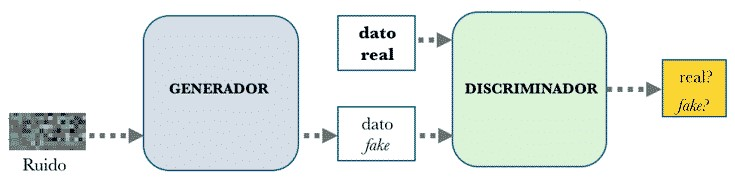
\includegraphics[scale = 0.5]{GANmodelo.jpg}
         \caption{Enfoques del Modelo Generador y Discriminador}
         \label{Alexis1}
       \end{center}
   \end{figure}
    

\end{frame}




\begin{frame}{SRGAN}

   \begin{block}{GAN}
      El termino \emph{Adversarial} se refiere a la dinámica 
      competitiva que se mantiene entre los dos modelos. Por un lado,
      el generador tiene por objetivo crear nuevos datos que sean indistinguibles del
      conjunto de entrenamiento, mientras que el discriminador debe poder ser capaz
      de distinguir cuáles son los datos creados y los reales.
   \end{block}
 
\end{frame}



\begin{frame}{Funcionamiento}
   \begin{figure}[H]
      \begin{center}
        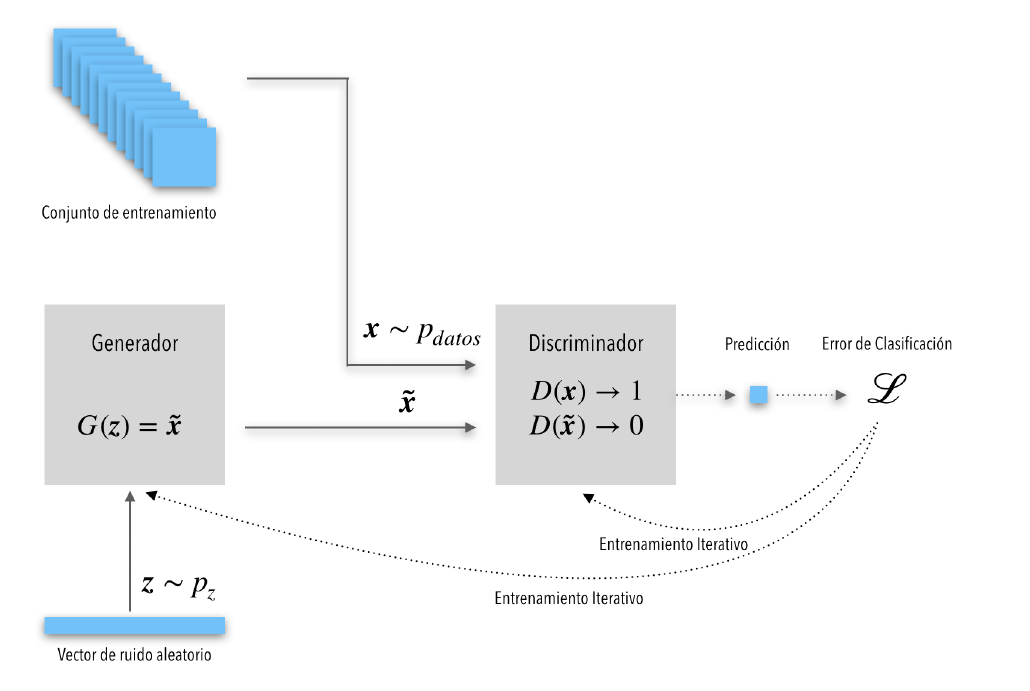
\includegraphics[scale = 0.5]{proceso_gan.png}
        \caption{Funciones del Modelo Generador y Discriminador}
        \label{Alexis2}
      \end{center}
   \end{figure}
   
\end{frame}

\begin{frame}{Desafios del modelo}
    
   \begin{block}{Principales fallas:}
       \begin{enumerate}
           \item  No convergencia:El generador y el discriminador no logran alcanzar un equilibrio.
           \item  Colapso modal:Esto ocurre cuando el generador produce muestras similares aunque las entradas sean de muy diversas características.
           \item  Pérdida no informativa: No es tan sencillo evaluar la mejora del modelo.
       \end{enumerate}
   \end{block}

\end{frame}

\begin{frame}{Funcionamiento}
   \begin{figure}[H]
      \begin{center}
        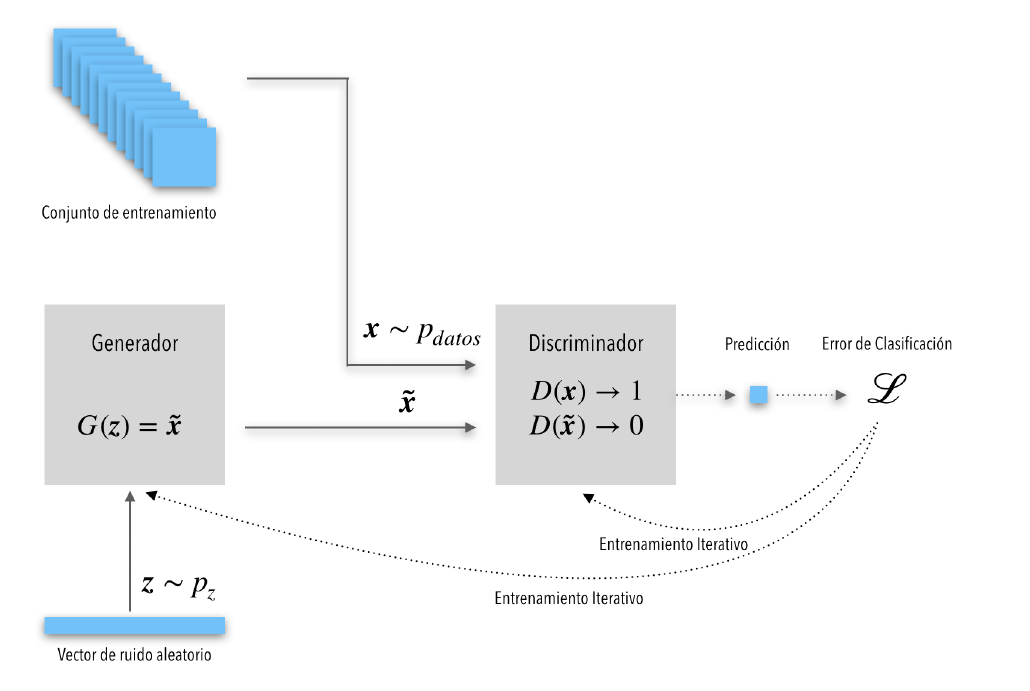
\includegraphics[scale = 0.5]{proceso_gan.png}
        \caption{Funciones del Modelo Generador y Discriminador}
        \label{Alexis9}
      \end{center}
   \end{figure}
   
\end{frame}